
\let\negmedspace\undefined
\let\negthickspace\undefined
\documentclass[journal]{IEEEtran}
\usepackage[a5paper, margin=10mm, onecolumn]{geometry}
%\usepackage{lmodern} % Ensure lmodern is loaded for pdflatex
\usepackage{tfrupee} % Include tfrupee package
\setlength{\headheight}{1cm} % Set the height of the header box
\setlength{\headsep}{0mm}     % Set the distance between the header box and the top of the text
\usepackage{gvv-book}
\usepackage{gvv}
\usepackage{cite}
\usepackage{amsmath,amssymb,amsfonts,amsthm}
\usepackage{algorithmic}
\usepackage{graphicx}
\usepackage{textcomp}
\usepackage{xcolor}
\usepackage{txfonts}
\usepackage{listings}
\usepackage{enumitem}
\usepackage{mathtools}
\usepackage{gensymb}
\usepackage{comment}
\usepackage[breaklinks=true]{hyperref}
\usepackage{tkz-euclide} 
\usepackage{listings}
% \usepackage{gvv}                                        
\def\inputGnumericTable{}                                 
\usepackage[latin1]{inputenc}                                
\usepackage{color}                                            
\usepackage{array}                                            
\usepackage{longtable}                                       
\usepackage{calc}                                             
\usepackage{multirow}                                         
\usepackage{hhline}                                           
\usepackage{ifthen}                                           
\usepackage{lscape}
\renewcommand{\thefigure}{\theenumi}
\renewcommand{\thetable}{\theenumi}
\setlength{\intextsep}{10pt} % Space between text and floats
\numberwithin{equation}{enumi}
\numberwithin{figure}{enumi}
\renewcommand{\thetable}{\theenumi}
\begin{document}
\bibliographystyle{IEEEtran}
\title{Question 3-3.3-12}
\author{EE24BTECH11015 - Dhawal}
% \maketitle
% \newpage
% \bigskip
{\let\newpage\relax\maketitle}
\begin{enumerate}
\item Construct a $\Delta ABC$ in which $AB=6cm,BC=8cm\text{ and } \angle{ABC}=\ang{60}$.

\end{enumerate}

\begin{table}[h!]    
  \centering
  
\begin{tabular}[12pt]{ |c| c| c|}
    \hline
    \textbf{Variable} & \textbf{Description} & \textbf{Values} \\ 
    \hline
    AB & Length & 6 cm \\
    \hline
    BC & Length & 8 cm \\
    \hline
    $\angle ABC$ & Angle & \ang{60}\\
    \hline 
    $\vec{A}$ & Point & $(6,0)$ \\
    \hline
    $\vec{B}$ & Origin & $(0,0)$ \\
    \hline
    $\vec{C}$ & To find & ? \\
    \hline
    \end{tabular}


  \caption{Variables given}
  \label{tab 1.4.9.2}
\end{table}
Solution:\\
As $AB=6cm$ put:
\begin{align}
       \vec{A}=\myvec{6\\0}, \vec{B}=\myvec{0\\0},
\end{align}
Then,
\begin{align}
	\vec{C}=\myvec{BC\cos{60\degree}\\BC\sin{60\degree}}=\myvec{4\\4\sqrt{3}}
\end{align}

\begin{figure}[h!]
   \centering
   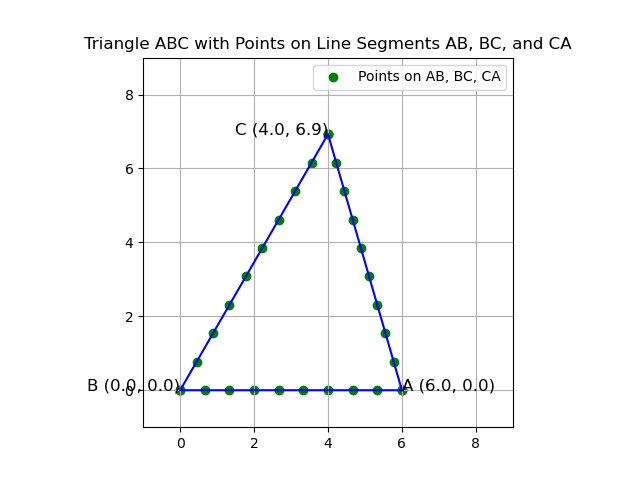
\includegraphics[width=1\linewidth]{Figure_1.png}
	\caption{$\Delta ABC$ }
   \label{stemplot}
\end{figure}


\end{document}

